\title{%
  The terminal: Pipes and redirects
}
\author{Daniel Bosk}
\institute{%
  KTH EECS
}

\mode<article>{\maketitle}
\mode<presentation>{%
  \begin{frame}
    \maketitle
  \end{frame}
}

\mode*


\section{What to learn?}

\begin{frame}
  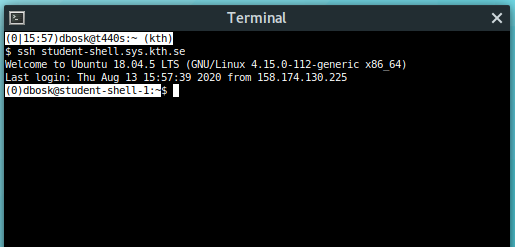
\includegraphics[width=\columnwidth]{../../ssh/terminal.png}
\end{frame}

\begin{frame}[fragile]
  \begin{lstlisting}[numbers=none]
cat hitch-hikers-guide.txt | \
  tr -cs A-Za-z '\n' | tr A-Z a-z | \
  sort | \
  uniq -c | \
  sort -rn | \
  head -n 10
  \end{lstlisting}
\end{frame}

\begin{frame}
  \begin{block}{What we've learned}
    \begin{description}
      \item[Navigation] \lstinline{pwd cd ls .. .}
      \item[Files] \lstinline{mkdir rmdir touch cp mv rm}
      \item[Contents] \lstinline{cat less head tail grep file nano}
    \end{description}
  \end{block}
\end{frame}


\section{Pipes}

\begin{frame}[fragile]
  \begin{block}<+->{Pipes and function composition}
    \begin{description}
      \item[Composition] \(
          (g \circ f)(x) = g(f(x))
        \)
      \item[Pipe] \lstinline{cat x | f | g}
    \end{description}
  \end{block}

  \begin{example}<+>[Counting words and lines]
    \begin{itemize}
      \item \lstinline{echo one | wc}
      \item \lstinline{echo -n one | wc}
      \item \lstinline{echo one two | wc}
      \item \lstinline{(echo one; echo two; echo three) | wc}
    \end{itemize}
  \end{example}
\end{frame}

\begin{frame}[fragile]
  \begin{example}<+>[Sorting lines]
    \begin{itemize}
      \item \lstinline{(echo one; echo two; echo three) | sort}
    \end{itemize}
  \end{example}

  \begin{example}<+>[Sorting lines and counting them]
    \begin{itemize}
      \item \lstinline{(echo one; echo two; echo three) | sort | wc}
    \end{itemize}
  \end{example}
\end{frame}

\begin{frame}[fragile]
  \begin{example}[Finding patterns]
    \begin{itemize}
      \item \lstinline{(echo one; echo two; echo three) | grep "e" | wc -l}
    \end{itemize}
  \end{example}
\end{frame}


\section{Redirections}

\begin{frame}[fragile]
  \begin{onlyenv}<1-3>
    \begin{block}{Data streams}
      \begin{description}
        \item[Output]
          standard output (stdout, screen),
          standard error (stderr, screen),
          file
        \item[Input]
          standard input (stdin, keyboard),
          file
      \end{description}
    \end{block}
  \end{onlyenv}

  \begin{example}<2>[stdin: ignored, stdout: terminal screen]
    \begin{lstlisting}
cat existingfile
    \end{lstlisting}
  \end{example}

  \begin{example}<3>[stdin: terminal keyboard, stdout: terminal screen]
    \begin{lstlisting}
cat
    \end{lstlisting}
  \end{example}

  \begin{onlyenv}<4>
    \begin{remark}[By default]
      \begin{itemize}
        \item stdin connected to terminal (keyboard).
        \item stdout connected to terminal (screen).
      \end{itemize}
    \end{remark}
  \end{onlyenv}
\end{frame}

\begin{frame}[fragile]
  \begin{example}<+>[stdin: ignored, stderr: terminal, stdout: file]
    \begin{lstlisting}
cat nonexistingfile > out.txt
    \end{lstlisting}
  \end{example}
\end{frame}

\begin{frame}[fragile]
  \begin{center}
    \lstinline[basicstyle=\LARGE]{> >> < <<}
  \end{center}
\end{frame}

\begin{frame}[fragile]
  \begin{example}<+>[stdout: file]
    \begin{lstlisting}
echo contents of file.txt > file.txt
    \end{lstlisting}
  \end{example}

  \begin{example}<+>[stdout: append to file]
    \begin{lstlisting}
echo more contents of file.txt >> file.txt
    \end{lstlisting}
  \end{example}
\end{frame}

\begin{frame}[fragile]
  \begin{example}<+>[stdin: ignored/file, stdout: terminal]
    \begin{lstlisting}
cat file.txt
cat < file.txt
    \end{lstlisting}
  \end{example}
\end{frame}

\begin{frame}[fragile]
  \begin{example}<+>[stdin: terminal, stdout: terminal]
    \begin{lstlisting}
(echo one; echo two; echo three) | wc -l
wc -l << _END
one
two
three
_END
    \end{lstlisting}
  \end{example}
\end{frame}

\begin{frame}
  \begin{center}
    \lstinline[basicstyle=\huge]{a | b}
  \end{center}
  \begin{remark}
    \begin{itemize}
      \item \lstinline{|} connects stdout of \lstinline{a} to stdin of 
        \lstinline{b}!
      \item stdout of \lstinline{b} connected to terminal (screen).
      \item stdin of \lstinline{a} connected to terminal (keyboard).
    \end{itemize}
  \end{remark}
\end{frame}


\section{An exercise}

\begin{frame}[fragile]
  \begin{block}<+>{What we've learned}
    \begin{description}
      \item[Navigation] \lstinline{pwd cd ls .. .}
      \item[Files] \lstinline{mkdir rmdir touch cp mv rm}
      \item[Contents] \lstinline{cat less head tail grep file nano}
      \item[Pipes, redir] \lstinline{| > >> < <<}
    \end{description}
  \end{block}

  \begin{exercise}
    \begin{itemize}
      \item Which commands must you run (and in which order) to get the same 
        output?
      \item But this time without using any text editor (such as 
        \lstinline{nano}).
    \end{itemize}
    \begin{lstlisting}[numbers=none]
$ grep "contents" testfiles2/testfile.txt
contents of testfile.txt
contents of testfile.txt
contents of testfile.txt
    \end{lstlisting}
  \end{exercise}
\end{frame}

\begin{frame}[fragile]
  \begin{solution}<+>[One alternative]
    \begin{lstlisting}
mkdir testfiles2
cp testfiles/testfile.txt testfiles2/
    \end{lstlisting}
  \end{solution}
  \begin{solution}<+>[A more interesting alternative]
    \begin{lstlisting}
mkdir testfiles2
echo contents of testfile.txt > testfiles2/testfile.txt
echo contents of testfile.txt >> testfiles2/testfile.txt
echo contents of testfile.txt >> testfiles2/testfile.txt
    \end{lstlisting}
  \end{solution}
\end{frame}

\begin{frame}[fragile]
  \begin{solution}<+>[An even more interesting alternative]
    \begin{lstlisting}
mkdir testfiles2
echo some garbage > testfiles2/testfile.txt
echo contents of testfile.txt >> testfiles2/testfile.txt
echo more garbage >> testfiles2/testfile.txt
echo contents of testfile.txt >> testfiles2/testfile.txt
echo contents of testfile.txt >> testfiles2/testfile.txt
echo more garbage >> testfiles2/testfile.txt
    \end{lstlisting}
  \end{solution}
\end{frame}

\begin{frame}[fragile]
  \begin{solution}<+>[Yet another alternative]
    \begin{lstlisting}
mkdir testfiles2
cat testfile.txt > testfiles2/testfile.txt
cat testfile.txt >> testfiles2/testfile.txt
cat testfile.txt >> testfiles2/testfile.txt
    \end{lstlisting}
  \end{solution}
  \begin{solution}<+>[Yet another]
    \begin{lstlisting}
mkdir testfiles2
cp testfile.txt testfiles2/
cat testfile.txt >> testfiles2/testfile.txt
cat testfile.txt >> testfiles2/testfile.txt
    \end{lstlisting}
  \end{solution}
\end{frame}

\begin{frame}[fragile]
  \begin{solution}<+>[The last one we'll give]
    \begin{lstlisting}
mkdir testfiles2
cd testfiles2
cp ../testfile.txt .
echo contents of testfile.txt >> testfile.txt
echo contents of testfile.txt >> ./testfile.txt
    \end{lstlisting}
  \end{solution}
\end{frame}


\section{Conclusion}

\begin{frame}[fragile]
  \begin{exercise}[What does this series of commands do?]
    \begin{lstlisting}[numbers=none]
cat hitch-hikers-guide.txt | \
  tr -cs A-Za-z '\n' | tr A-Z a-z | \
  sort | \
  uniq -c | \
  sort -rn | \
  head -n 10
    \end{lstlisting}
  \end{exercise}
\end{frame}

\begin{frame}
  \begin{solution}[McIlroy's solution]
    \begin{itemize}
      \item \lstinline{cat} just provides contents of 
        \lstinline{hitch-hikers-guide.txt}.
      \item \lstinline{tr -cs} turns all characters other than A--Z and a-z 
        into \lstinline{\\n} (new line, meaning all words are on their own 
        line).
      \item \lstinline{tr} turns all words into lower case (translates A--Z 
        into a--z).
      \item \lstinline{sort} sorts all lines (words).
      \item \lstinline{uniq -c} counts each word and outputs counts.
      \item \lstinline{sort -rn} sorts in reverse order and numerical values 
        (not alphabetical).
      \item \lstinline{head -n 10} takes 10 first lines, ignores the rest.
    \end{itemize}
  \end{solution}
\end{frame}

\begin{frame}[fragile]
  \begin{exercise}
    \begin{itemize}
      \item Use \lstinline{join} and \lstinline{cut} (and the commands you 
        already know) to make a list of name and phone number sorted on last 
        name.
    \end{itemize}
    names.csv: \lstinputlisting{names.csv}

    phone.csv: \lstinputlisting{phone.csv}

    \pause

    Expected result:
    \begin{lstlisting}[numbers=none]
Fritjof,Adamsson,072-1234567
Adam,Bertilsson,071-1234567
Daniel,Bosk,070-1234567
    \end{lstlisting}
  \end{exercise}
\end{frame}

\begin{frame}[fragile]
  \begin{solution}[One possible solution]
    \lstinputlisting{phonebook.sh}
  \end{solution}
\end{frame}


%%% REFERENCES %%%

%\begin{frame}[allowframebreaks]
%  \printbibliography{}
%\end{frame}
